\documentclass[a4paper,11pt]{article}
\usepackage[utf8]{inputenc}
\usepackage[spanish]{babel}
\usepackage[affil-it]{authblk}
\usepackage{enumerate}
\usepackage{graphicx}
\usepackage{listings}
\usepackage{hyperref}
\usepackage{amsmath}
\usepackage{amssymb}
\usepackage{cancel}
\usepackage[usenames, dvipsnames]{color}
\usepackage{tikz}
\usepackage[labelfont=bf]{caption}
\usepackage{subcaption} %Multiple images
\usepackage{multicol} % Multiple columns
\usepackage{float}
\usepackage{cleveref}
\usepackage{relsize} % bigger math symbols
\usepackage[margin=1.1in]{geometry}
\usepackage[titletoc,toc,title]{appendix}
\usepackage{enumitem}
\usepackage{etoolbox}
\usepackage{mdframed} %frame theorems
\usetikzlibrary{calc}
\numberwithin{equation}{section}

% Footnotes with symbols

\makeatletter
\def\@fnsymbol#1{\ensuremath{\ifcase#1\or \dagger\or \ddagger\or
   \mathsection\or \mathparagraph\or \|\or **\or \dagger\dagger
   \or \ddagger\ddagger \else\@ctrerr\fi}}
\makeatother

\renewcommand{\thefootnote}{\fnsymbol{footnote}}

%Styling for code
\definecolor{codegreen}{rgb}{0,0.6,0}
\definecolor{codegray}{rgb}{0.5,0.5,0.5}
\definecolor{codepurple}{rgb}{0.58,0,0.82}
\definecolor{backcolour}{rgb}{0.95,0.95,0.92}
 
\lstdefinestyle{mystyle}{
    backgroundcolor=\color{backcolour},   
    commentstyle=\color{codegreen},
    keywordstyle=\color{magenta},
    numberstyle=\tiny\color{codegray},
    stringstyle=\color{codepurple},
    basicstyle=\footnotesize,
    breakatwhitespace=false,         
    breaklines=true,                 
    captionpos=b,                    
    keepspaces=true,                 
    numbers=left,                    
    numbersep=5pt,                  
    showspaces=false,                
    showstringspaces=false,
    showtabs=false,                  
    tabsize=2
}
 
\lstset{style=mystyle}

% Cool letters 
%Filename:      Typocaps.fd
%Created by:    MLO
%Creation date: 2003/04/02

% This file should be put in a TeX input directory

\ProvidesFile{Typocaps.fd}
   [2003/04/02 Font definition file for U/Typocaps]

\DeclareFontFamily{U}{Typocaps}{}

\DeclareFontShape{U}{Typocaps}{xl}{n}{
   <-> Typocaps
}{}

\endinput


% Footer
\usepackage{fancyhdr}
\pagestyle{fancy}
\fancyhf{}
\cfoot{\fontsize{15pt}{15pt}\usefont{U}{Typocaps}{xl}{n} 
gigantium humeris insidentes}

% Big Pictures
\usepackage[export]{adjustbox}

% Enviroment for theorems
\newmdtheoremenv[frametitle=Teorema]{theo}{Theorem}

% Circled words
\newcommand{\circled}[2][]{%
  \tikz[baseline=(char.base)]{%
    \node[shape = circle, draw, inner sep = 1pt]
    (char) {\phantom{\ifblank{#1}{#2}{#1}}};%
    \node at (char.center) {\makebox[0pt][c]{#2}};}}
\robustify{\circled}

%Appendices in spanish
\renewcommand{\appendixname}{Ap\'endices}
\renewcommand{\appendixtocname}{Ap\'endices}
\renewcommand{\appendixpagename}{Ap\'endices}

%Zero delimiter
\newcommand{\zerodel}{.\kern-\nulldelimiterspace}

%Columns separation
\setlength{\columnsep}{1cm}

%Indentation
\setlength{\parindent}{0ex}

%Multiple References

\crefrangelabelformat{equation}{(#3#1#4--#5\crefstripprefix{#1}{#2}#6)}

\usepackage{xparse}

%Boxes

\newcommand*{\boxcolor}{blue}
\makeatletter
\renewcommand{\boxed}[1]{\textcolor{\boxcolor}{%
\tikz[baseline={([yshift=-1ex]current bounding box.center)}] \node [rectangle, minimum width=1ex,rounded corners,draw] {\normalcolor\m@th$\displaystyle#1$};}}
 \makeatother

%Constantes
\newcommand{\euler}{\mathrm{e}}
\newcommand{\im}{i}

%Lemas, teoremas, definiciones y pruebas
\newcommand{\definicion}{\textbf{Definición: }}
\newcommand{\lema}{\textbf{Lema: }}
\newcommand{\teorema}{\textbf{Teorema: }}
\newcommand{\prueba}{\textbf{Prueba: }}
\newcommand{\proposicion}{\textbf{Proposición: }}
\newcommand{\corolario}{\textbf{Corolario: }}

% Definición de las secciones y su numeración

\makeatletter
\def\@seccntformat#1{%
  \expandafter\ifx\csname c@#1\endcsname\c@section\else
  \csname the#1\endcsname\quad
  \fi}
\makeatother

\begin{document}

\begin{titlepage}
\thispagestyle{fancy}

\newcommand{\HRule}{\rule{\linewidth}{0.5mm}} % Defines a new command for the horizontal lines, change thickness here

\center % Center everything on the page
 
%----------------------------------------------------------------------------------------
%	HEADING SECTIONS
%----------------------------------------------------------------------------------------

\textsc{\LARGE Universidad Nacional Autónoma de México}\\[0.3cm] % Name of your university/college

%----------------------------------------------------------------------------------------
%	LOGO SECTION
%----------------------------------------------------------------------------------------


\includegraphics[scale=0.17]{unam}

%----------------------------------------------------------------------------------------
%	SUBHEADING SECTIONS
%----------------------------------------------------------------------------------------

\textsc{\Large Electrodinámica Clásica}\\[0.3cm] % Major heading such as course name
\textsc{\large Semestre 2016-II}\\[0.3cm] % Minor heading such as course title
\textsc{\large 12 de mayo de 2016}\\ % Date

%----------------------------------------------------------------------------------------
%	TITLE SECTION
%----------------------------------------------------------------------------------------

\HRule \\[0.1cm]
{ \huge \bfseries Tarea \# 9. \\ Radiación.}\\ % Title of your document
\HRule \\[0.1cm]
 
%----------------------------------------------------------------------------------------
%	AUTHOR SECTION
%----------------------------------------------------------------------------------------
\setcounter{footnote}{0}
\center
\large
\emph{Autor:} \\ % Your name
\Large Favio \textsc{Vázquez}\footnote[1]{\href{mailto:favio.vazquez@correo.nucleares.unam.mx}{favio.vazquez@correo.nucleares.unam.mx}}
\\[0.7cm]
%----------------------------------------------------------------------------------------
%	COOL IMAGE SECTION
%----------------------------------------------------------------------------------------

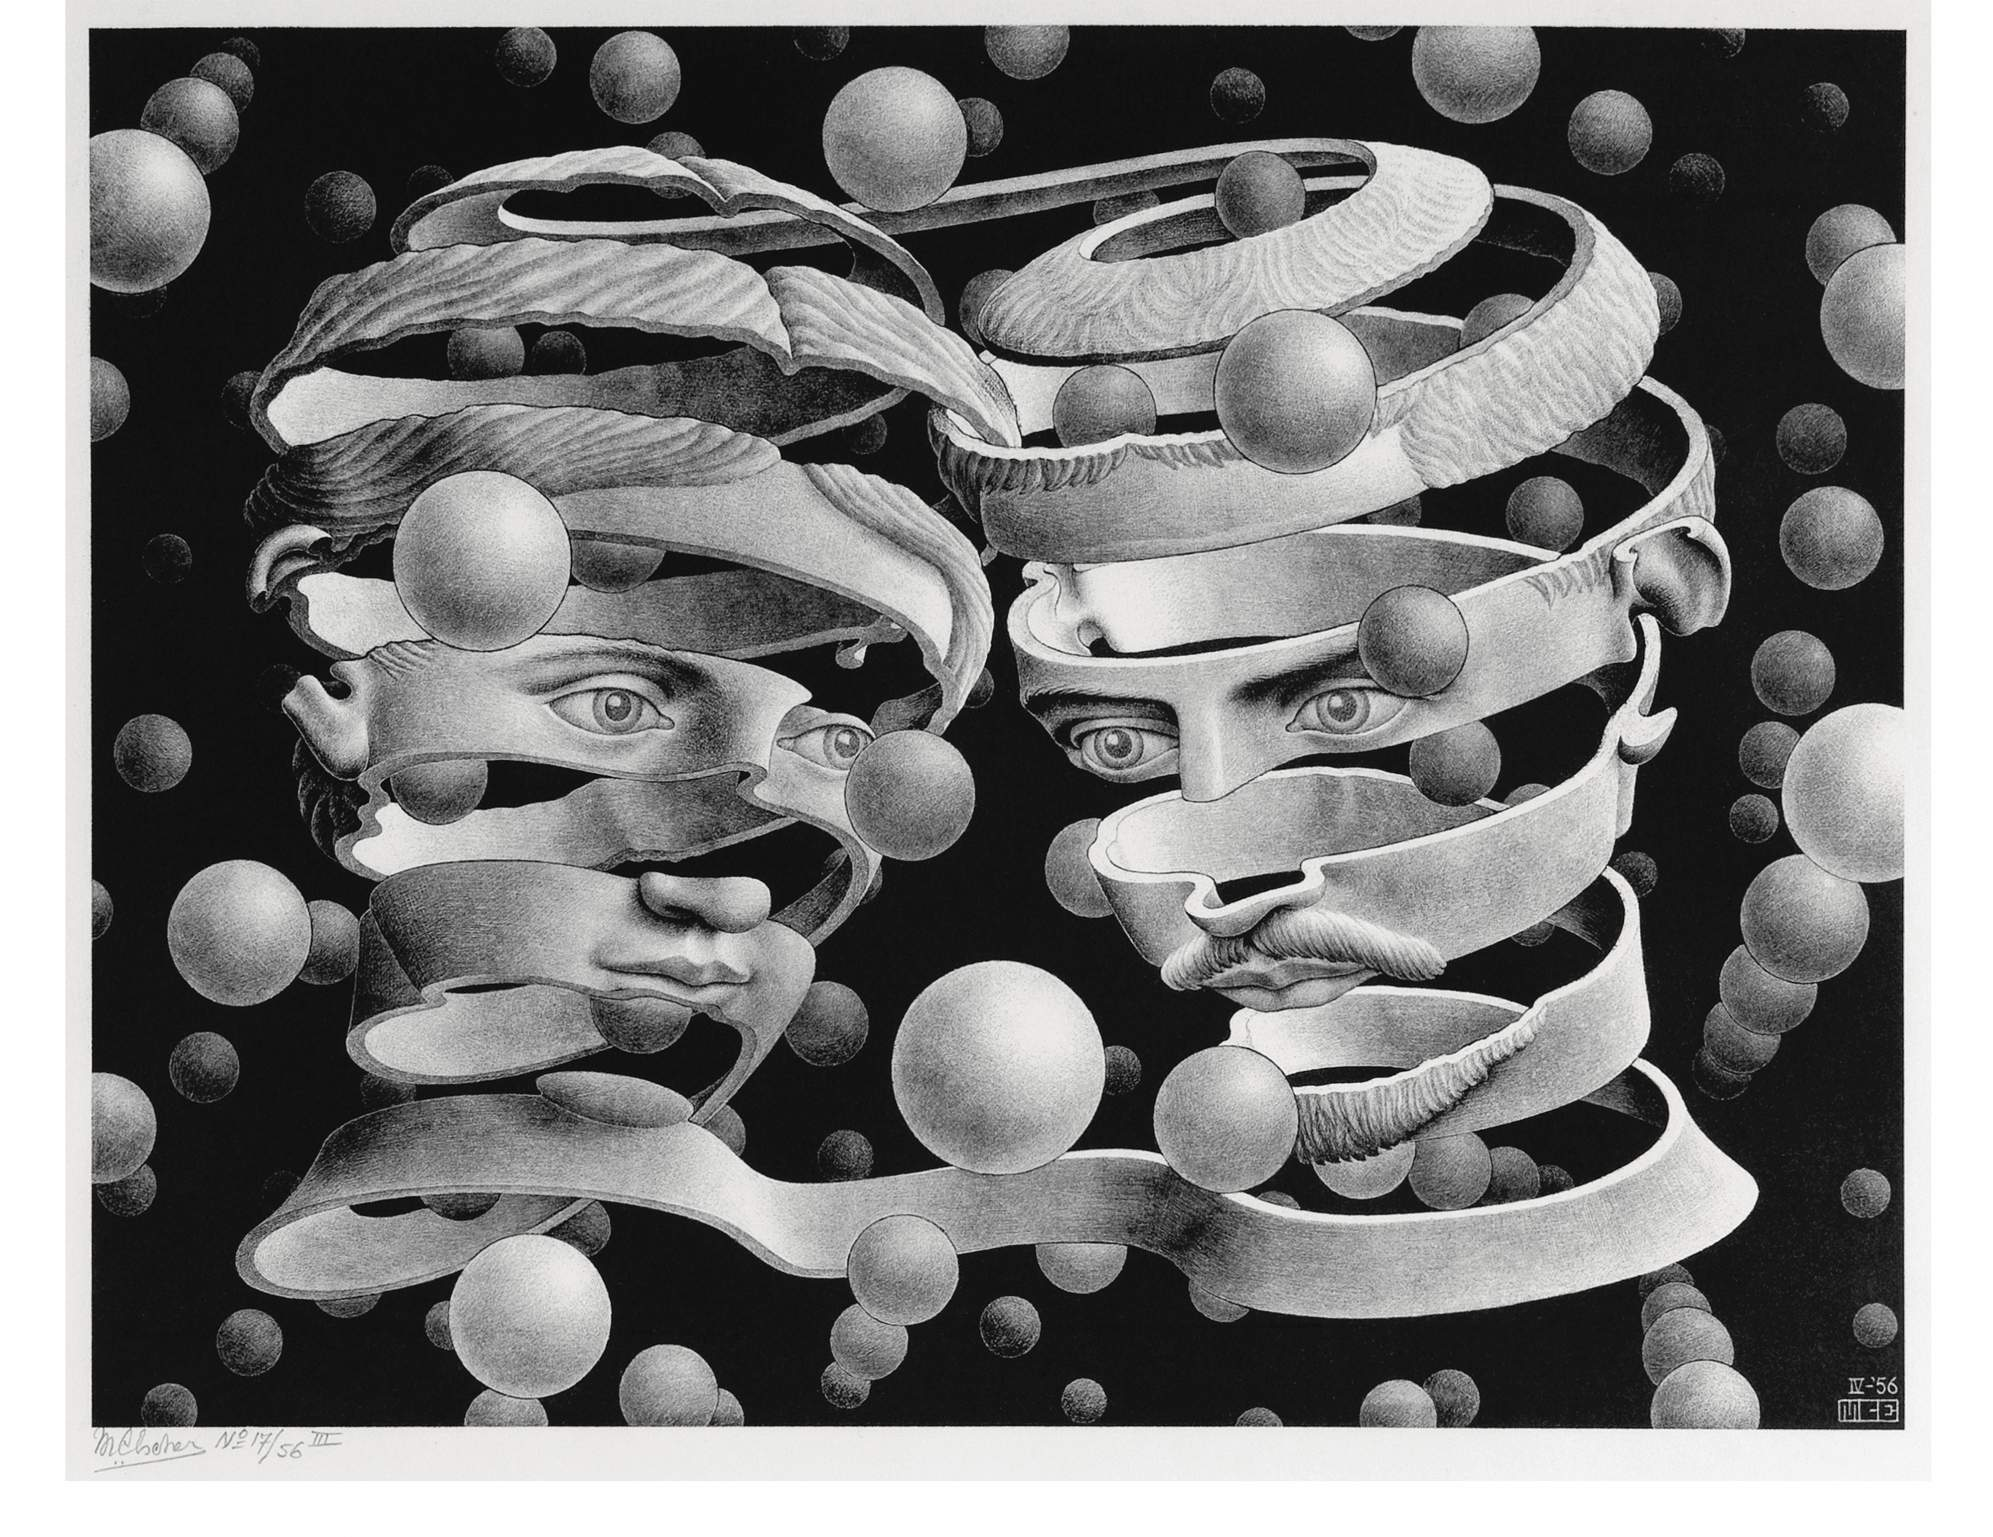
\includegraphics[scale=0.56]{escherCaras}

%----------------------------------------------------------------------------------------

\vfill % Fill the rest of the page with whitespace

\end{titlepage}

% ---------------------------------------------------------------------------------------
%         HEADER
%----------------------------------------------------------------------------------------

\fancyhead[L]{Favio Vázquez}
\fancyhead[R]{\thepage}

%----------------------------------------------------------------------------------------
\setcounter{footnote}{0}
\renewcommand*{\thefootnote}{\arabic{footnote}}
%----------------------------------------------------------------------------------------

%----------------------------------------------------------------------------------------
%%			BEGIN DOCUMENT
%----------------------------------------------------------------------------------------

\section{Problema 1}

En la zona lejana demostrar, partiendo de los potenciales retardados, 

\begin{enumerate}[label=\textbf{(\alph*)}]
 \item 
 
 $$
 \mathbf{A} = \frac{\dot{\mathbf{p}}}{cr} + \frac{\dot{\mathbf{m}} \times 
 \hat{n}}{cr} + \frac{\ddot{Q}_{\alpha}}{6c^2r}, \quad \text{donde} \quad
 Q_\alpha = Q_{\alpha\beta} \hat{n}_\beta
 $$
 
 \item 
 
 $$
 P = \frac{2|\ddot{p}|^2}{3c^3} + \frac{2|\ddot{m}|^2}{3c^3} +
 \frac{\ddot{Q}_{\alpha\beta}}{180c^5}.
 $$
\end{enumerate}

\underline{Solución:} \vspace{.3cm}

Esta demostración se hará a partir de Landau y Lifshitz \cite{landau}, por lo 
tanto la notación será la de ese texto. Para entender la notación del texto 
comenzamos con la sección $\S 66$. Como trabajamos para la zona lejana, consideremos 
el campo producida por un sistema de cargas móviles a distancias que son grandes 
comparadas con la dimensiones del sistema. 

\vspace{.3cm}

Elijamos, como el autor, el origen de coordenadas $O$ en un punto cualquiera interior 
al sistema de cargas. Llamemos $R_0$ el vector de origen en $O$ y extremo en el 
punto de observación del campo, $P$, y sea $\mathbf{n}$ el vector unitario 
correspondiente. Sea $\mathbf{r}$ el vector posición del elemento de carga 
$de = \rho dV$ y $\mathbf{R}$ el vector de origen en $de$ y extremo en $P$. 
Evidentemente, $\mathbf{R} = \mathbf{R}_0 - \mathbf{r}$. 

\vspace{.3cm}

A grandes distancias del sistema, es $R_0 \gg r$ y se tiene aproximadamente: 

\begin{equation}
 R = |\mathbf{R}_0 - \mathbf{r}| \approx R_0 - \mathbf{r} \cdot \mathbf{r}.
\end{equation}

Con esta notación, el potencial vectorial retardado, donde el tiempo retardado 
es $t' = t - \frac{R}{c}$, 

\begin{equation}
 \mathbf{A} = \frac{1}{cR_0}\int \mathbf{J}_{t' + \frac{\mathbf{r}\cdot\mathbf{n}}{c}} dV,  
\end{equation}

y si ahora desarrollamos en potencias de $\mathbf{r}\cdot \mathbf{n}/c$, y 
conservando ahora los dos primeros términos se encuentra;

\begin{equation}
 \mathbf{A} = \frac{1}{cR_0} \int \mathbf{J}_{t'}dV + \frac{1}{c^2R_0} 
 \frac{\partial}{\partial t'} \int (\mathbf{r} \cdot \mathbf{n})\mathbf{J}_{t'} dV.
\end{equation}

Sustituyendo $\mathbf{J} = \rho \mathbf{v}$ y pasando a cargas puntuales, obtenemos:

\begin{equation}
 \mathbf{A} = \frac{\sum e \mathbf{v}}{cR_0} + \frac{1}{c^2R_0}\frac{\partial}{\partial t}
 \sum e \mathbf{v} (\mathbf{r} \cdot \mathbf{n}).
\end{equation}

Desde aquí, como hace el libro en la sección $\S 71$, prescindimos del índice $t'$
para simplificar la notación. En el segundo término de la ecuación anterior 
hagamos 

\begin{align*}
 \mathbf{v}(\mathbf{r} \cdot \mathbf{n}) &= \frac{1}{2} \frac{\partial}{\partial t}
 \mathbf{r}(\mathbf{n} \cdot \mathbf{r}) + \frac{1}{2}\mathbf{v}(\mathbf{n} \cdot \mathbf{r})
 - \frac{1}{2}\mathbf{r}(\mathbf{n} \cdot \mathbf{v})
 &=  \frac{1}{2} \frac{\partial}{\partial t}\mathbf{r}(\mathbf{n} \cdot \mathbf{r})
 + \frac{1}{2} (\mathbf{r} \times \mathbf{v}) \times \mathbf{n}.
\end{align*}

Se encuentra entonces para $\mathbf{A}$ la expresión 

\begin{equation}
 \mathbf{A} = \frac{\dot{\mathbf{d}}}{cR_0} + \frac{1}{2c^2R_0}\frac{\partial^2}{ 
 \partial t^2} \sum e \mathbf{r} (\mathbf{n} \cdot \mathbf{r}) + \frac{1}{cR_0} 
 (\dot{m} \times \mathbf{n}),
\end{equation}

donde $\mathbf{d}$ es el momento dipolar del sistema y $\mathbf{m} = \frac{1}{2c} 
\sum e \mathbf{r} \times \mathbf{v}$ es su momento magnético. Para seguir la 
transformación, podemos observar, sin cambiar el campo, podemos sumar a $\mathbf{A}$ 
un a $\mathbf{A}$ un vector cualquiera proporcional a $\mathbf{n}$. Entonces 
nos queda 

\begin{equation}
 \mathbf{A} = \frac{\dot{\mathbf{d}}}{cR_0} + \frac{1}{2c^2R_0}\frac{\partial^2}{ 
 \partial t^2}\sum e[3\mathbf{r}(\mathbf{n} \cdot \mathbf{r}) - \mathbf{n}r^2] + 
 \frac{1}{cR_0} \dot{m} \times \mathbf{n}.
\end{equation}

Pero la expresión que sigue al signo de derivación $\frac{\partial^2}{ 
\partial t^2}$ es precisamente el producto que dice el enunciado $Q_{\alpha\beta}n_\beta$ 
del vector $\mathbf{n}$ por el tensor momento cuadrupolar $Q_{\alpha\beta} = 
\sum r (3x_\alpha x\_beta - \delta_{\alpha\beta}r^2)$, entonces encontramos la 
expresión para el potencial vectorial 

\begin{equation}
 \mathbf{A} = \frac{\dot{\mathbf{d}}}{cR_0} + \frac{1}{cR_0}\dot{m}\times \mathbf{n} + 
 \frac{1}{6c^2R_0}\ddot{Q}_\alpha,
\end{equation}

que podemos escribir en la notación del problema haciendo $R_0 \rightarrow r$ y 
con un poco de álgebra vectorial como 

\begin{equation}
 \boxed{\mathbf{A} = \frac{\dot{\mathbf{p}}}{cr} + \frac{\dot{\mathbf{m}} \times 
 \hat{n}}{cr} + \frac{\ddot{Q}_{\alpha}}{6c^2r}, \quad \text{donde} \quad
 Q_\alpha = Q_{\alpha\beta} \hat{n}_\beta}.
\end{equation}

\hspace{10cm}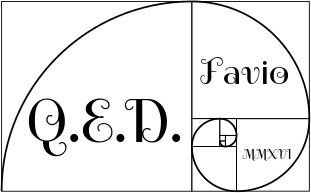
\includegraphics[scale=0.25]{logoQED}

\textbf{(b)} Ahora la intensidad de potencia emitida en el ángulo sólido $d\Omega$ 
viene dada por 

\begin{equation}
 dP = c \frac{H^2}{4\pi}r^2 d\Omega,
\end{equation}

y dado que a partir del potencial retardado en la expansión multipolar para zona 
lejana podemos encontrar que (ec. 71.4) 

\begin{equation}
 \mathbf{H} = \frac{1}{c^2r}\left(\ddot{d} \times \mathbf{n} + 
 \frac{1}{6c}\dddot{\mathbf{Q}} \times \mathbf{n} + 
 (\ddot{m} \times \mathbf{n}) \times \mathbf{n}\right),
\end{equation}

podemos calcular la potencia radiada total, es decir, la energía radiada por el sistema 
en todas direcciones por unidad de tiempo. Para ello, se determina el valor medio 
de $dP$ para todas las direcciones de $\mathbf{n}$; la potencia total es igual 
a este valor medio multiplicado por $4\pi$. Al promediar el cuadrado del 
campo magnético, se anulan todos los productos cruzados en los tres términos de 
$\mathbf{H}$, de forma que sólo los valores medios de los cuadrados de cada uno de 
ellos. Obtenemos entonces 

\begin{equation}
 \mathbf{P} = \frac{2}{3c^3}\ddot{\mathbf{d}}^2 + \frac{2}{3c^3}\ddot{m}^2 + 
 \frac{1}{180c^5}\ddot{Q}^2_{\alpha\beta},
\end{equation}

que podemos escribir como, con un poco de álgebra vectorial, 

\begin{equation}
 \boxed{P = \frac{2|\ddot{p}|^2}{3c^3} + \frac{2|\ddot{m}|^2}{3c^3} +
 \frac{\ddot{Q}_{\alpha\beta}}{180c^5}}.
\end{equation}

\hspace{10cm}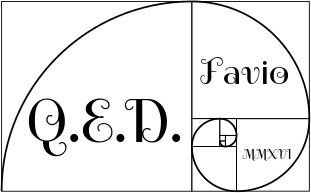
\includegraphics[scale=0.25]{logoQED}

\section{Problema 2}

Explicar la radiación de bremsstrahlung.

\vspace{.3cm} \underline{Solución:} \vspace{.3cm}

Los cálculos para esta sección se harán en S.I. ya que se tomaron en gran parte
de la sección 23.3 de Zangwill \cite{zangwill}. Lo que trabajaremos será con 
la teoría clásica de bremsstrahlung, y veremos que solo es un nombre a que se 
le da a un tipo de radiación en electrodinámica.

\vspace{.3cm}

La energía radiada al infinito por una partícula cargada está determinada por 
los campos de aceleración $\mathbf{E}_a(\mathbf{r},t)$ y $\mathbf{B}_a(\mathbf{r},t)$ 
fueron obtenidos en la tarea anterior, acá los escribimos en S.I. para trabajar con 
ellos 

\begin{equation}
 \mathbf{E}_a(\mathbf{r},t) = \frac{q}{4\pi\epsilon_0}\left[\frac{\hat{n} 
 \times \{(\hat{n} - \pmb{\beta}) \times \dot{\pmb{\beta}} \}}{cg^3R} \right]_{ret},
\end{equation}

\begin{equation}
 \mathbf{B}_a(\mathbf{r},t) = \frac{\mu_0q}{4\pi}\left[\frac{(\pmb{\beta} \times 
 \hat{n})(\dot{\pmb{\beta}} \cdot \hat{n}) + g\dot{\pmb{\beta}} 
 \times \hat{n}}{g^3R} \right]_{ret},
\end{equation}

donde $\pmb{\beta} = \mathbf{v}/c$, $g(t') = \frac{d}{dt}[r' - r + R(t')/c]$ y 
$\hat{n}$ es un vector unitario definido por $\mathbf{R}(t) = R(t)\hat{n}(t)$ y 
el $ret$ se refiere a que las mediciones se hacen el tiempo retardado. 

\vspace{.3cm}

Éstos son campos de radiación porque decrecen con $1/R$ y forman una triada 
ortogonal con el vector unitario retardado de la línea de visión, $\hat{n}_{ret}$. 
El vector de Poynting asociado, 

\begin{equation}
 \mathbf{S}(t) = \frac{1}{\mu_0}\mathbf{E}_a \times \mathbf{B}_a = 
 \epsilon_0cE_{a}^2 \hat{n}_{ret} = \epsilon_0c\left(\frac{q}{4\pi\epsilon_0}\right)^2 
 \left|\frac{\hat{n} \times [(\hat{n} - 
 \pmb{\beta} \times \dot{\pmb{\beta}})]}{cg^3R}\right|_{ret} \hat{n}_{ret}, 
\end{equation}

determina la tasa en la cual la energía fluye a través de un ángulo sólido $d\Omega$ 
de una esfera envolvente distante de radio $R$:

\begin{equation}
 \frac{dP(t)}{d\Omega} = \frac{dU}{dtd\Omega} = R^2 \mathbf{S}(t) \cdot \hat{n}_{ret}.
\end{equation}

La tasa de emisión se convierte en una cantidad más fundamental cuando 
la multiplicamos por $g_{ret}$ y nos enfocamos en la distribución angular del 
poder emitido, 

\begin{equation}
 \frac{dP(t)}{d\Omega} = \frac{dU}{dt_{ret}d\Omega} = g_{ret} R^2 \mathbf{S}(t) 
 \cdot \hat{n}_{ret} = \frac{1}{c}\left(\frac{q}{4\pi\epsilon_0}\right)^2 
 \left|\frac{\hat{n} \times [(\hat{n} - 
 \pmb{\beta} \times \dot{\pmb{\beta}})]}{(1 - \hat{n}\cdot \pmb{\beta})^5}\right|_{ret}.
\end{equation}

Esta ecuación se simplifica considerablemente cuando la aceleración $\mathbf{a}$ es 
paralela a la velocidad $\mathbf{v}$. El patrón de radiación tiene simetría 
azimutal al rededor su dirección común y entonces depende solamente del 
ángulo $\theta$ definido por $\hat{n} \cdot \pmb{\beta} = (v/c)\cos{\theta}$. 
Recordando que todas las cantidades se refieren al tiempo retardado de 
emisión, la distribución angular de la radiación emitida es 

\begin{equation}
 \left\zerodel \frac{dP}{d\Omega}\right|_{\parallel} = \frac{\mu_0q^2}{16\pi^2c} 
 \frac{a^2\sen^{\theta}}{(1 - \beta\cos{\theta})^5}.
\end{equation}

Ahora la dependencia de esta ecuación en $a^2$ nos dice que el patrón de radiación 
ocurre cuando la carga se acelera o se desacelera. La palabra alemana bremsstrahlung 
que significa ``radiación de frenado'' es usada comúnmente para el caso de desaceleración. 
Un ejemplo de la teoría clásica de bremsstrahlung es cuando un electrón de rápida 
velocidad choca con un blanco metálico, y se desacelera rápidamente, dando lugar a 
este tipo de radiación, bremsstrahlung \cite{griffiths}.

\section{Problema 3}

Para una partícula no relativista acelerada dibujar el patrón de radiación.

\vspace{.3cm} \underline{Solución:} \vspace{.3cm}

Para solucionar este problema recrearemos la figura 9.5 de Jackson \cite{jackson} que 
a nuestro parecer representa varios aspectos de los patrones de radiación. En la 
sección 9.9 del texto, el autor describe como se llegan a las ecuaciones para 
poder encontrar los patrones de radiación tanto dipolares como cuadrupolares, 
y dispone una tabla donde se encuentran distribuciones angulares para la forma 
normalizada del vector de armónicos esféricos $\mathbf{X}_{lm}(\theta,\phi)$, que 
se define como (ec. 9.119 de Jackson \cite{jackson})

\begin{equation}
 \mathbf{X}_{lm}(\theta,\phi) = \frac{1}{\sqrt{l(l+1)}}\mathbf{L}Y_{lm}(\theta,\phi),
\end{equation}

donde $\mathbf{L} = \frac{1}{i}(r \times \pmb{\nabla})$. La tabla en cuestión 
es la siguiente (tabla 9.1 de Jackson \cite{jackson})

\begin{figure}[H]
 \center 
 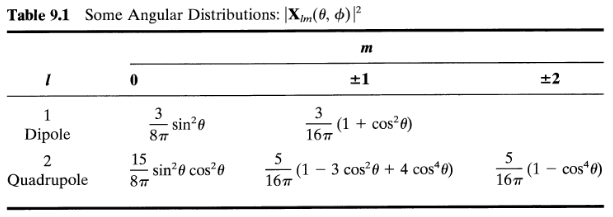
\includegraphics[scale=0.5]{problema3fig1}
\end{figure}

Debajo las distribuciones dipolares se ven como aquellas en las que un dipolo 
oscila paralelo al eje $z$ ($m=0$) y las que dos dipolos, uno a lo largo del eje 
$x$ y otro a lo largo del eje $y$, $90^\circ$ fuera de fase ($m = \pm 1)$. Las 
distribuciones angulares dipolares y cuadrupolares están graficadas 
debajo como diagramos de intensidad dipolar. Representan distribuciones angulares 
para $l=1$ y $l=2$. La ecuación de donde salen las porciones de ecuaciones que 
se encuentran en la tabla de arriba es la (9.152) de Jackson \cite{jackson}. Cada 
una tiene su respectiva leyenda que la relaciona a la tabla de arriba, y la última 
figura es un compendio de todos los patrones de radiación.

\begin{figure}[H]
 \center
 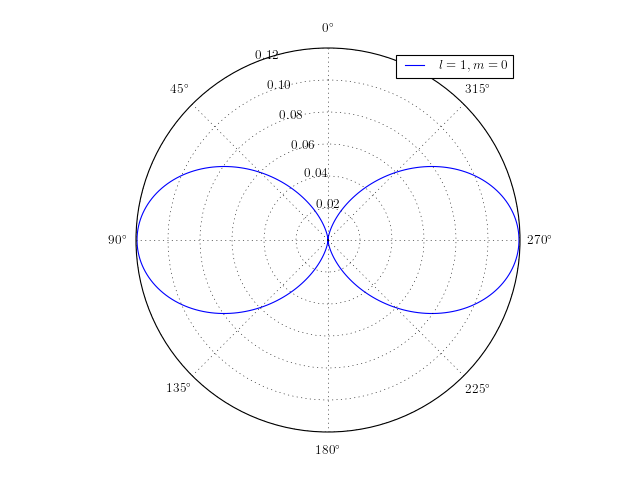
\includegraphics[scale=0.6]{problema3fig2}
\end{figure}

\begin{figure}[H]
 \center
 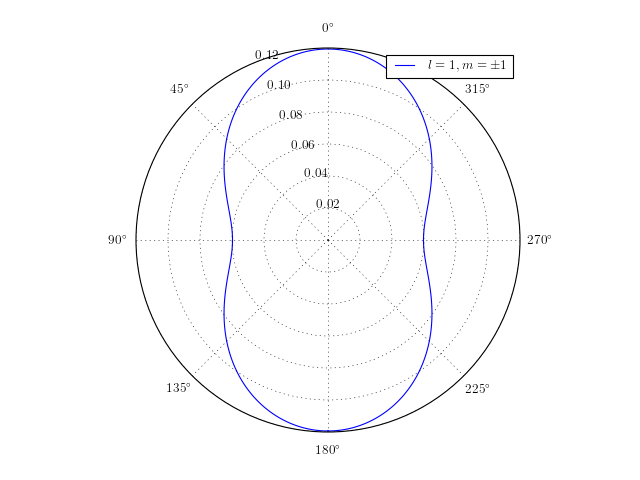
\includegraphics[scale=0.6]{problema3fig3}
\end{figure}

\begin{figure}[H]
 \center
 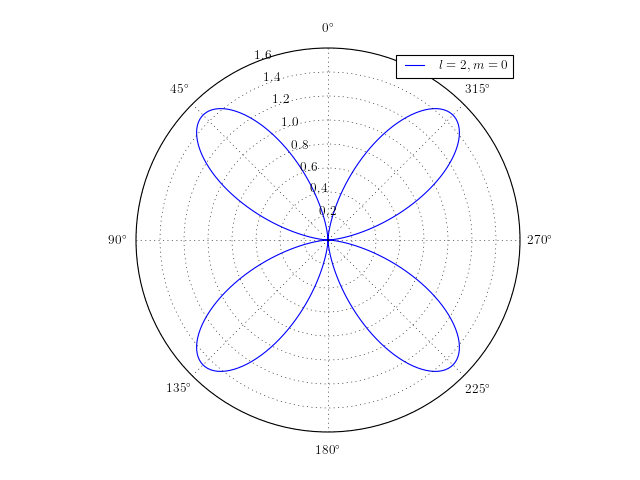
\includegraphics[scale=0.6]{problema3fig4}
\end{figure}

\begin{figure}[H]
 \center
 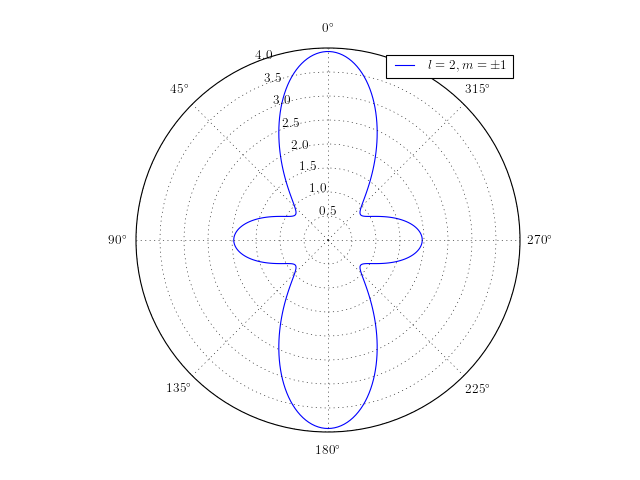
\includegraphics[scale=0.6]{problema3fig5}
\end{figure}

\begin{figure}[H]
 \center
 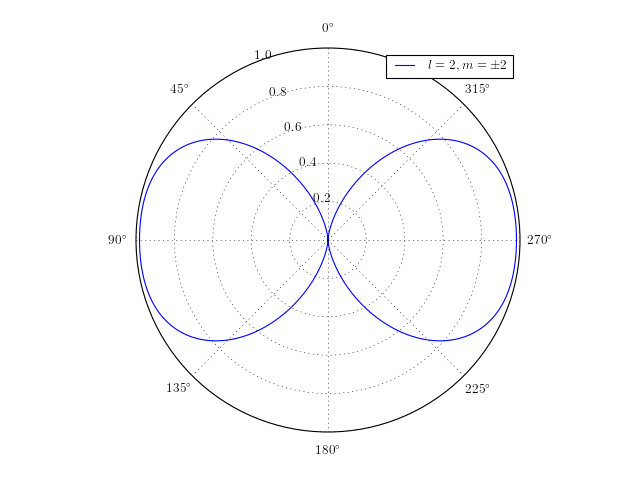
\includegraphics[scale=0.6]{problema3fig6}
\end{figure}

El código que hace estas imágenes de arriba es 
(\href{https://github.com/FavioVazquez/Electrodinamica-Clasica-PCF/blob/master/Tarea9/Problema3.ipynb}{Link al 
notebook de Python en mi GitHub})

\begin{lstlisting}[language=Python]
from __future__ import print_function
import numpy as np
from numpy import arccos,sin, cos, pi, array, sqrt, log, exp
import matplotlib
matplotlib.use('nbagg')
import matplotlib.pyplot as plt
from matplotlib import rc

rc('font',**{'family':'sans-serif','sans-serif':['Helvetica']})
## for Palatino and other serif fonts use:
#rc('font',**{'family':'serif','serif':['Palatino']})
rc('text', usetex=True)

#LaTeX
plt.rc('text', usetex=True)
plt.rc('font', family='serif')

# Linespace for theta

theta = np.linspace(-pi,pi,360)

# Variable definitions
x1 = 3/(8*pi)*(sin(theta))**2 #l=1,m=0
x2 = 3/(16*pi)*(1 + (cos(theta))**2)#l=1,m=+-1
x3 = 15/8*pi * (sin(theta))**2*(cos(theta))**2 #l=2,m=0
x4 = (5/8*pi) * (1 - 3*(cos(theta))**2 + 
             4*(cos(theta))**4) #l=2, m=+-1
x5= 5/16*pi * (1 - (cos(theta))**4)

#Plots and Style

# l=1, m=0
ax = plt.subplot(111, polar=True)
ax.set_theta_offset(pi/2)
ax.plot(theta,x1,label=r'$l=1,m=0$')
ax.legend(loc=1,fontsize=12)
plt.show()

# l=1, m=+-1 
ax = plt.subplot(111, polar=True)
ax.set_theta_offset(pi/2)
ax.plot(theta,x2,label=r'$l=1,m=\pm 1$')
ax.legend(loc=1,fontsize=12)
plt.show()

# l=2, m=0
ax = plt.subplot(111, polar=True)
ax.set_theta_offset(pi/2)
ax.plot(theta,x3, label=r'$l=2,m=0$')
ax.legend(loc=1,fontsize=12)
plt.show()

# l=2, m=+-1
ax = plt.subplot(111, polar=True)
ax.set_theta_offset(pi/2)
ax.plot(theta,x4, label=r'$l=2,m=\pm 1$')
ax.legend(loc=1,fontsize=12)
plt.show()

# l=2, m=+-2
ax = plt.subplot(111, polar=True)
ax.set_theta_offset(pi/2)
ax.plot(theta,x5, label=r'$l=2,m=\pm 2$')
ax.legend(loc=1,fontsize=12)
plt.show()
\end{lstlisting}

Compendio de patrones de radiación

\begin{figure}[H]
 \center
 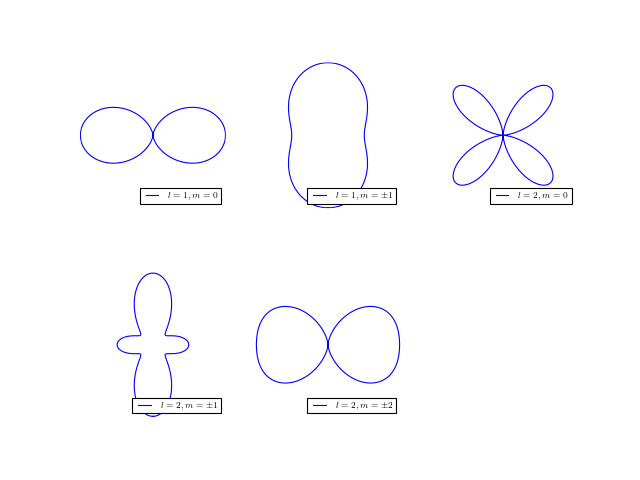
\includegraphics[scale=0.62]{problema3fig7}
\end{figure}

El código que hace esta figura es 

\begin{lstlisting}[language=Python]
 from __future__ import print_function
import numpy as np
from numpy import arccos,sin, cos, pi, array, sqrt, log, exp
import matplotlib
matplotlib.use('nbagg')
import matplotlib.pyplot as plt
from matplotlib import rc

rc('font',**{'family':'sans-serif','sans-serif':['Helvetica']})
## for Palatino and other serif fonts use:
#rc('font',**{'family':'serif','serif':['Palatino']})
rc('text', usetex=True)

#LaTeX
plt.rc('text', usetex=True)
plt.rc('font', family='serif')

# Linespace for theta

theta = np.linspace(-pi,pi,360)

# Variable definitions
x1 = 3/(8*pi)*(sin(theta))**2 #l=1,m=0
x2 = 3/(16*pi)*(1 + (cos(theta))**2)#l=1,m=+-1
x3 = 15/8*pi * (sin(theta))**2*(cos(theta))**2 #l=2,m=0
x4 = (5/8*pi) * (1 - 3*(cos(theta))**2 + 
             4*(cos(theta))**4) #l=2, m=+-1
x5= 5/16*pi * (1 - (cos(theta))**4)

fig = plt.figure()

#Plots
ax1 = fig.add_subplot(231,projection='polar')
ax1.plot(theta,x1,label=r'$l=1,m=0$')
ax2 = fig.add_subplot(232,projection='polar')
ax2.plot(theta,x2,label=r'$l=1,m=\pm 1$')
ax3 = fig.add_subplot(233,projection='polar')
ax3.plot(theta,x3, label=r'$l=2,m=0$')
ax4 = fig.add_subplot(234,projection='polar')
ax4.plot(theta,x4, label=r'$l=2,m=\pm 1$')
ax5 = fig.add_subplot(235,projection='polar')
ax5.plot(theta,x5, label=r'$l=2,m=\pm 2$')

#Offsets
ax1.set_theta_offset(pi/2)
ax2.set_theta_offset(pi/2)
ax3.set_theta_offset(pi/2)
ax4.set_theta_offset(pi/2)
ax5.set_theta_offset(pi/2)

#Legends
ax1.legend(loc=4,fontsize=8)
ax2.legend(loc=4,fontsize=8)
ax3.legend(loc=4,fontsize=8)
ax4.legend(loc=4,fontsize=8)
ax5.legend(loc=4,fontsize=8)

#Axis style
ax1.axis('off')
ax2.axis('off')
ax3.axis('off')
ax4.axis('off')
ax5.axis('off')

plt.show()
\end{lstlisting}

\section{Problema 4}

¿Cuánto tiempo tarda en caer un electrón al núcleo? Considere el átomo de hidrógeno 
y n=1.

\vspace{.3cm} \underline{Solución:} \vspace{.3cm}

La pérdida de energía dominante en este caso está dada por la radiación dipolar, 
que utilizando la ecuación de Larmor podemos escribir como 

\begin{equation}
 \frac{dU}{dt} = - \langle P \rangle = - \frac{2a^2e^2\omega^4}{3c^3}.
 \label{eq:161}
\end{equation}

Para un electrón de carga $-e$ y masa $m_e$ en una órbita de radio $a$ acerca 
de un núcleo fijo de carga $+e$ (átomo de hidrógeno), la segunda ley de Newton, 
$F=ma$ nos dice que 

\begin{equation}
 \frac{e^2}{a^2} = m \frac{v^2}{a} = m\omega^2a,
\end{equation}

de manera que 

\begin{equation}
 \omega^2 = \frac{e^2}{ma^3},
 \label{eq:163}
\end{equation}

y también la energía total será 

\begin{equation}
 U = - \frac{e^2}{a} + \frac{1}{2}mv^2 = - \frac{e^2}{2a}.
 \label{eq:164}
\end{equation}

Usando las ecuaciones \eqref{eq:163} y \eqref{eq:164} en la ecuación \eqref{eq:161}, 
tenemos 

\begin{equation}
 \frac{dU}{dt} = \frac{e^2}{2a^2} \dot{a} = - \frac{2e^6}{3a^4m^2c^3},
\end{equation}

o 

\begin{equation}
 a^2\dot{a} = \frac{1}{3} \frac{da^3}{dt} = - \frac{4e^4}{3m^2c^3} = - \frac{4}{3}r_0^2c,
\end{equation}

donde $r_0 = e^2/mc^2$ es el radio clásico del electrón. Entonces 

\begin{equation}
 a^3 = a_0^3 - 4r_0^2ct.
\end{equation}

El tiempo de caída del electrón será entonces ($a \rightarrow 0$) 

\begin{equation}
 t_{\text{caída}} = \frac{a_0^3}{4r_0^2c}.
\end{equation}

Sustituyendo los valores conocidos para $r_0 = 2.8 \times 10^{-13}$ cm y 
$a_0 = 5.3 \times 10^{-9}$ cm, el tiempo de caída del electrón al núcleo será 
$\boxed{t_{\text{caída}} = 1.6 \times 10^{-11} s}$. Este es el orden de magnitud para el tiempo de 
vida de un átomo de hidrógeno excitado con $n=1$.

\begin{thebibliography}{10}
\bibitem{landau}
L. Landau y E. Lifshitz, \emph{Teoría Clásica de los campos}, Vol. 2 del Curso de 
Física Teórica, 2da edición, 1992.
 \bibitem{zangwill}
 A. Zangwill, \emph{Modern Electrodynamics}, Cambridge University Press, 2012.
 \bibitem{griffiths}
 D. Griffits, \emph{Introduction to Electrodynamics}, 4ta edición, Pearson Education, 
 2013.
 \bibitem{jackson}
J. Jackson, \emph{Classical Electrodynamics}, 3ra edición. John Wiley and Sons, Inc. 
1999.
\end{thebibliography}


\end{document}